%%\documentstyle[twocolumn,jsaiac]{jarticle}
%%\documentstyle[twocolumn,jsaiac]{j-article}
\documentclass[twocolumn]{jarticle}

\usepackage{color}
\usepackage{multirow}
\usepackage{subcaption}
\usepackage[dvipdfmx]{graphicx}
\usepackage{jsaiac}
\usepackage{bm}

%%
\title{
\jtitle{Masked Language Modeling を用いた}
\jtitle{Knowledge Graph 補完手法の検討}
\etitle{Investigating Knowledge Graph Completion Techniques Using Masked Language Modeling}
}
%%英文は以下を使用
%\title{Style file for manuscripts of JSAI 20XX}

\jaddress{堀本 隆誠,大阪府立大学 工学域,大阪府堺市中区学園町 1-1,seb01120@st.osakafu-u.ac.jp}

\author{%
\jname{堀本 隆誠\first}
\ename{Ryusei Horimoto}
\and
\jname{岡田 真 \second}
\ename{Makoto Okada}
\and
\jname{森 直樹\second}
\ename{Naoki Mori}
%Given-name Surname\third{}%%英文は左を使用
}

\affiliate{
\jname{\first{大阪府立大学}}
\ename{Osaka Prefecture University}
\and
\jname{\second{大阪公立大学}}
\ename{Osaka Metropolitan University}
%\and
%\third{}Affiliation \#3 in English%%英文は左を使用
}

%%
%\Vol{28}        %% <-- 28th(変更しないでください)
%\session{0A0-00}%% <-- 講演ID(必須)

\begin{abstract}
In recent years, with the rapid development of artificial intelligence technology, Knowledge Graph, which systematically connects various kinds of human knowledge and expresses their relationships in a graph structure, has attracted much attention and is used as a fundamental technology for artificial intelligence in various fields. In this context, there is a need for an automatic complementation method of Knowledge Graphs to meet the demand for adding new knowledge to existing Knowledge Graphs. The problem with conventional Knowledge Graph completion methods such as TransE and ComplEx is that they focus on knowledge relationships and do not effectively capture the semantic information of the knowledge itself. In this study, we proposed an automatic Knowledge Graph completion method using Masked Language Modeling by BERT, which is a deep language model, to effectively capture the semantic information of knowledge itself, and verified its effectiveness through evaluation experiments. 
\end{abstract}

%\setcounter{page}{1}
\def\Style{``jsaiac.sty''}
\def\BibTeX{{\rm B\kern-.05em{\sc i\kern-.025em b}\kern-.08em%
 T\kern-.1667em\lower.7ex\hbox{E}\kern-.125emX}}
\def\JBibTeX{\leavevmode\lower .6ex\hbox{J}\kern-0.15em\BibTeX}
\def\LaTeXe{\LaTeX\kern.15em2$_{\textstyle\varepsilon}$}

\begin{document}
\maketitle

\vspace{-1mm}
\section{はじめに}

近年, 人工知能技術は急速な発展を遂げている. その中で人間の知識をグラフ構造で表現する Knowledge Graph \cite{kg} が注目を集めており, 人工知能の基盤技術としてさまざまな分野で活用されている. Knowledge Graph はさまざまな知識とそのつながりをグラフ構造を用いて表現するデータ構造である. 多種多様な情報とそのつながりを体系的に表現できるという利点や, 数値や有限の属性値に限らず自然言語文や音声データといった非構造データを情報として扱えるという利点がある. これらの利点は, ある情報においてそれにつながるさまざまな知識が得られるという点で 1 つの概念に対する情報を得たいときに有用である. しかし, Knowledge Graph 内の知識とそれらの関係を人手ですべて網羅するには多大なコストがかかる. この問題を解決するために Knowledge Graph 内の関係を基に含まれていない関係を自動的に補完する手法が求められている. 従来の Knowledge Graph 補完手法である TransE \cite{TransE_WN18} や ComplEx \cite{ComplEx} などの問題点として,知識の関係性を重視して学習しており, 知識自体の意味情報を効果的に捉えていない点がある.\par
本研究では,知識自体の意味情報を効果的に捉えるために深層言語モデルである BERT による Masked Language Modeling を用いた Knowledge Graph 自動補完手法を提案して,評価実験によりその有効性を検証した. \par

\vspace{-1mm}
\section{要素技術}

\vspace{-1mm}
\subsection{Knowledge Graph}

Knowledge Graph \cite{kg} とは, さまざまな知識を体系的に連結し, その関係をグラフ構造で表した知識ネットワークのことである. 図 \ref{kg} に Knowledge Graph の例を示す. Knowledge Graph は, head, tail を要素に持つ entity 集合と, その entity 間の関係を表現する relation を要素に持つ relation 集合によって構成されており, 図 \ref{kg} のように entity をノード, relation をエッジとする有向グラフとして表される. また, Knowledge Graph を表す表現方法として (head, relation, tail) という 3 つ組構造(triple)の集合で表すこともできる. \par
Knowledge Graph はさまざまな種類のデータを統合的にグラフとして扱うため, 一度に多元的な情報を得ることができる. Knowledge Graph が利用されているものとして最も有名なものが Google Knowledge Graph \cite{google_knowledge_graph} である. これは Google が保有する各情報を entity として, それぞれが relation によって紐付けられた Knowledge Graph である. これを用いることでユーザーはある情報について検索した際にそれに付随する人や場所, 物事等に関する多角的な情報を得ることができる. \par

\begin{figure}[t]
    \centering
    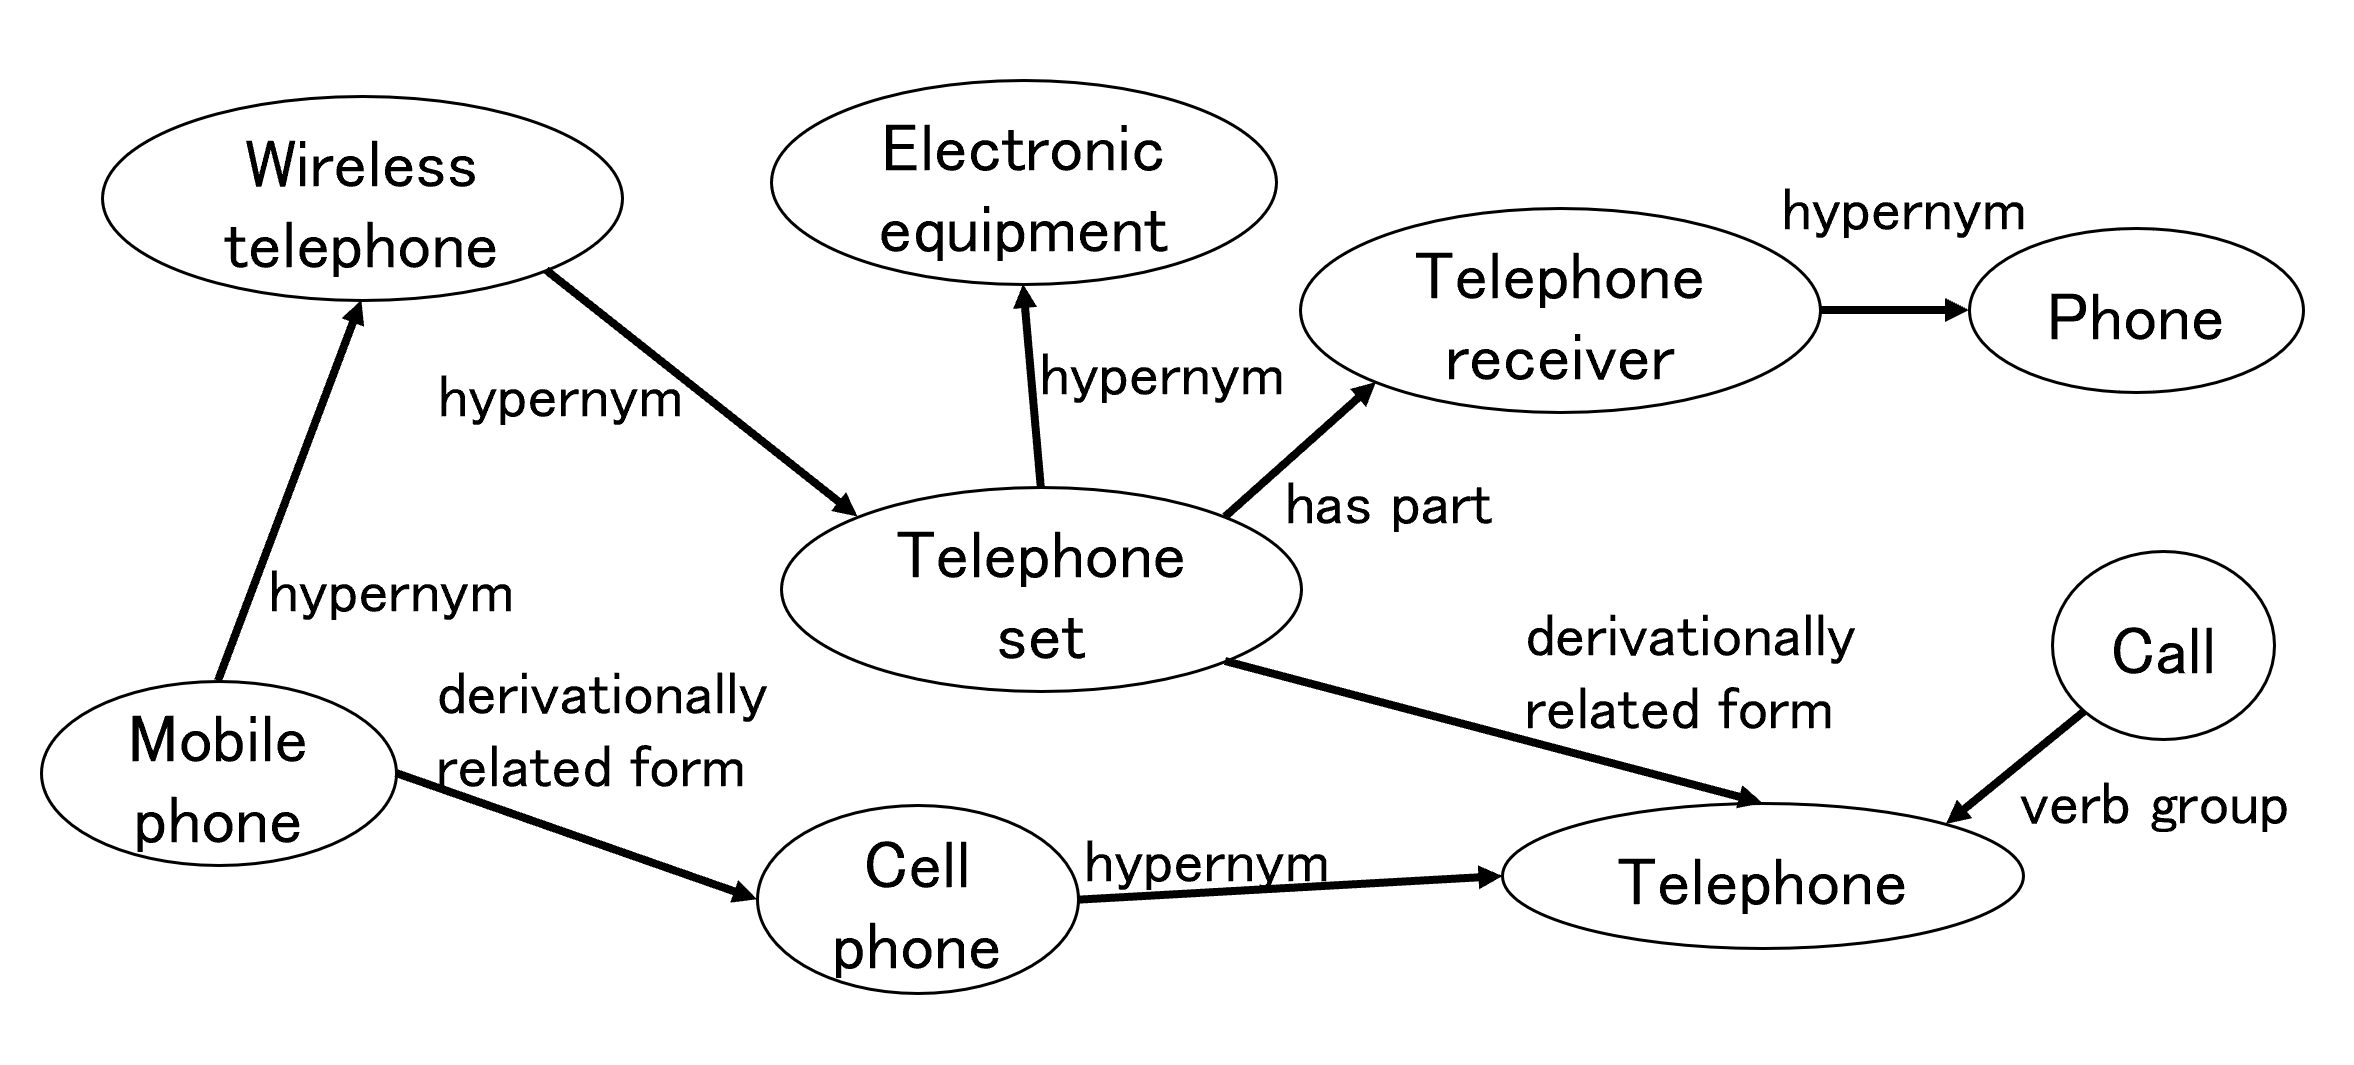
\includegraphics[width=80mm]{assets/Ex_KG.png}
    \vspace{-4mm}
    \caption{Knowledge Graph の例}
    \label{kg}
\end{figure}

\vspace{-1mm}
\subsection{BERT}

Bidirectional Encoder Representations from Transformers (BERT) \cite{BERT} は, 2018 年に Google が発表した Transformer をベースとして双方向エンコーダで構成された言語モデルである. BERT は入力された単語列全体とそれに含まれる各単語に対応する分散表現を出力する. また, BERT は膨大なデータを用いて 2 種類の教師なし学習をした事前学習済みモデルである. これを各タスクに fine-tuning することでさまざまなタスクに対応することができる. \par
学習には 2 つの文が連続するかを分類する Next Sentence Prediction (NSP) と, 入力データの一部の単語を ``[MASK]" トークンに置き換えて入力とし, 得られた各単語の分散表現から ``[MASK]" トークン部分の単語の元の単語を予測する Masked Language Modeling (MLM) がある. MLM において, ``[MASK]" に入る単語が何なのかを周辺の文脈から推定するタスクを解くことで, 文脈を考慮した単語埋め込みを生成する能力を獲得する. しかし, ``[MASK]" というトークンは事前学習には登場するものの, fine-tuning の際にはタスクによっては登場せず, 事前学習と fine-tuning に乖離が生じてしまう. その問題を緩和するため, ``[MASK]" トークンに置き換えた単語に対して, 一定の確率で元の単語に戻し, また一定の確率でランダムな単語に置き換える. BERT が提案された論文では, 入力トークンの 15\% のうち, 80\% を ``[MASK]" トークンに, 10\% をランダムなトークンに置き換え, 10\% を元のトークンのままにしている. \par

\vspace{-1mm}
\subsection{KG-BERT}

Knowledge Graph BERT (KG-BERT) \cite{KG-BERT} は, BERT を用いた Knowledge Graph 補完手法の 1 つであり, Yao らによって提案された. 図 \ref{KG-BERT} に KG-BERT モデルの概略図を示す. KG-BERT では, Knowledge Graph の head, relation, tail を ``[SEP]" トークンで区切ったものを BERT の入力として, その triple が存在するか否かを ``[CLS]" トークンのみを利用した 2 値分類で判定している. 学習の際は 1 つの triple に対してその tail を他の entity と置換した triple を 5 つ生成してそれらが存在しない triple だと判定するように学習する. テストの際は 1 つのテスト triple に対してその tail を他の entity と置換した triple を entity の数だけ生成し, それらの triple の分類スコアを順位付けすることで評価している. \par

\begin{figure}[t]
    \centering
    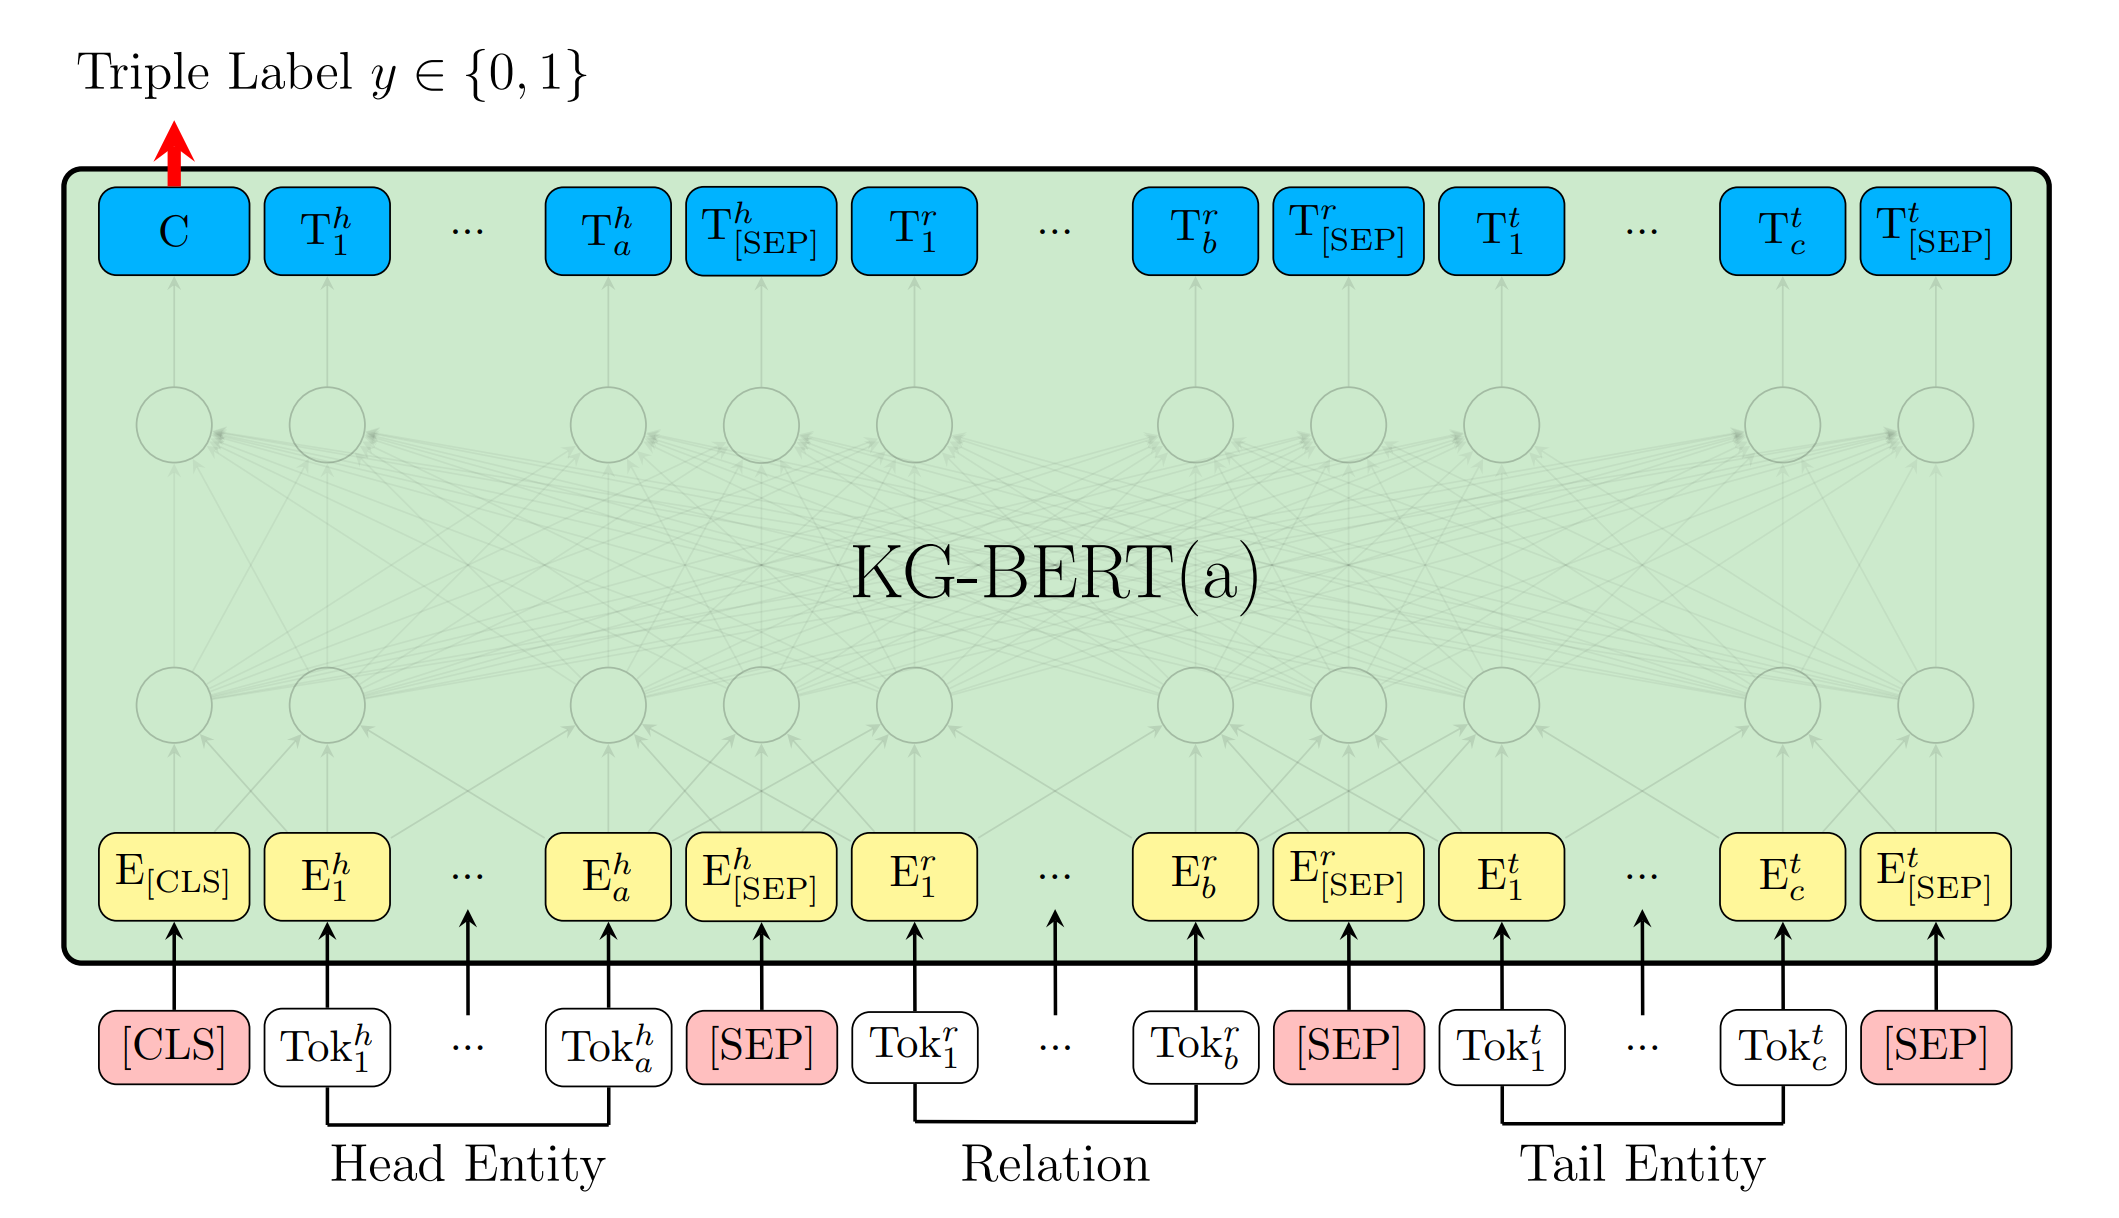
\includegraphics[width=85mm]{assets/KG-BERT.png}
    \vspace{-5mm}
    \caption{KG-BERT (文献 \cite{KG-BERT} 図 1 より参照)}
    \label{KG-BERT}
\end{figure}

\begin{table}[t]
    \centering
    \caption{WN18 から逆関係の triple を除去する例}
    \vspace{-3mm}
    \label{example_wn18}
    \scalebox{0.90}{
    \begin{tabular}{|c|c|c||c|} \hline
      head & relation & tail & \\ \hline \hline
      poodle dog & hypernym & domestic dog & \\
      domestic dog & hyponym & poodle dog & 除去 \\ \hline
      telephone & hypernym & telecommunicate & \\
      telecommunicate & hyponym & telephone & 除去 \\ \hline
      home movie & hypernym & picture show & \\
      picture show & hyponym & home movie & 除去 \\ \hline
      \vdots & \vdots & \vdots & \\ \hline
    \end{tabular}
    }
\end{table}

\vspace{-1mm}
\subsection{WN18RR}

WN18RR \cite{wn18rr} は, 英語の大規模な語彙データベースである WordNet \cite{wordnet} から triple を自動抽出して得られたデータセット WN18 \cite{TransE_WN18} を基に作成された triple のデータセットである. WordNet では, 単語同士の関係が品詞別に階層構造の形で格納されており, entity が単語の意味に対応し, relation が entity 間の語彙的な関係を表している. WN18 は WordNet のサブセットであり, ある triple に対してその逆関係の triple を含んでいる. WN18RR はその逆関係の triple を除去して得られたデータセットである. 表 \ref{example_wn18} に WN18 から逆関係の triple を除去する例を示す. triple (``poodle dog", ``hypernym", ``domestic dog"), (``domestic dog", ``hyponym", ``poodle dog") は逆関係の triple であるため, 後者の triple を WN18 から除去する. WN18RR では, entity は ``見出し語, その説明文" の形で表される. 表 \ref{example_entity}, \ref{example_wn18rr} に WN18RR における entity の例と WN18RR の例をそれぞれ示す. なお, 表 \ref{example_wn18}, \ref{example_wn18rr} では entity の説明文を省略して記述している. \par

\begin{table}[t]
    \centering
    \caption{WN18RR における entity の例}
    \vspace{-3mm}
    \label{example_entity}
    \scalebox{0.75}{
    \begin{tabular}{|cc|} \hline
      caption&description \\ \hline \hline
      poodle dog& an intelligent dog with a heavy curly solid-colored …\\
      domestic dog&a member of the genus Canis (probably descended …\\
      telephone&get or try to get into communication (with …\\
      wireless telephone&a telephone that communicates by radio waves …\\
      telephone set&electronic equipment that converts sound into …\\ \hline
      \multicolumn{2}{|c|}{\vdots} \\ \hline
    \end{tabular}
    }
\end{table}

\begin{table}[t]
    \centering
    \caption{WN18RR の例}
    \vspace{-3mm}
    \label{example_wn18rr}
    \scalebox{0.75}{
    \begin{tabular}{|c|c|c|} \hline
      head & relation & tail \\ \hline \hline
      telephone & hypernym & telecommunicate \\
      telephone system&has part&telephone set\\
      telephone system&has part&telephone exchange\\
      telephone system&hypernym&communication system \\
      telephone set&derivationally related form &telephone \\
      call&verb group&telephone \\
      cell phone&hypernym&telephone \\ \hline
      \vdots & \vdots & \vdots \\ \hline
    \end{tabular}
    }
\end{table}

\vspace{-1mm}
\section{提案手法}

Knowledge Graph の triple における head, relation, tail をそれぞれ h, r, t とすると, Knowledge Graph 補完では triple (h, r, t) に対して ``t" に入る tail を回答することで entity 間の関係性を予測する. 従来の Knowledge Graph 補完手法として Knowledge Graph Embedding 手法である TransE \cite{TransE_WN18} や ComplEx \cite{ComplEx} などがある. これらの手法は entity と relation をそれぞれ実数値ベクトルとして表し, それらのベクトルの関係式を用いて triple の妥当性を評価する. 例えば TransE では, まず entity と relation をそれぞれ $d$ 次元の埋め込み表現にする. このとき, 与えられる埋め込み表現はランダムに初期化されたベクトルとする. 次に triple を構成する head, relation, tail の埋め込み表現 $v_{\rm h}$, $v_{\rm r}$, $v_{\rm t}$ に対して, すべての triple が ``$v_{\rm h} + v_{\rm r} = v_{\rm t}$" を満たすように埋め込み表現を学習する. これにより head と relation から tail を予測することができる.このように, 既存の Knowledge Graph 補完手法は triple の構造情報を重視した手法となっており, entity 自体の意味情報を重視して補完する形ではないという特徴が挙げられる. \par
本研究では, entity 自体の意味情報を効果的に捉えるために BERT を MLM で fine-tuning したモデルを用いて, 1 つのシーケンス (head, relation, [MASK]) を入力文として tail を予測することによる Knowledge Graph 補完手法を提案する. 図 \ref{KG-MLM} に提案手法のモデル概略図を示す. BERT を MLM で fine-tuning するとき, BERT が提案された論文と同様に入力トークンの 15\% のうち, 80\% を ``[MASK]" トークンに置き換え, 10\% をランダムなトークンに置き換え, 10\% をそのままのトークンにする. さらに, 入力トークンの 15\% に tail の見出し語を必ず含むように設定する. 図 \ref{MLM_fine_tuning} に BERT の MLM による fine-tuning の概略図を示す. 図 \ref{KG-MLM}, \ref{MLM_fine_tuning} の Tok はトークンを, $E$, $T$ は埋め込みベクトルとモデルの出力のベクトルを示す. $l, m, n$ は head, relation, tail のトークン数を, h, r, t は head, relation, tail をそれぞれ表す.  \par

\begin{figure}[t]
    \centering
    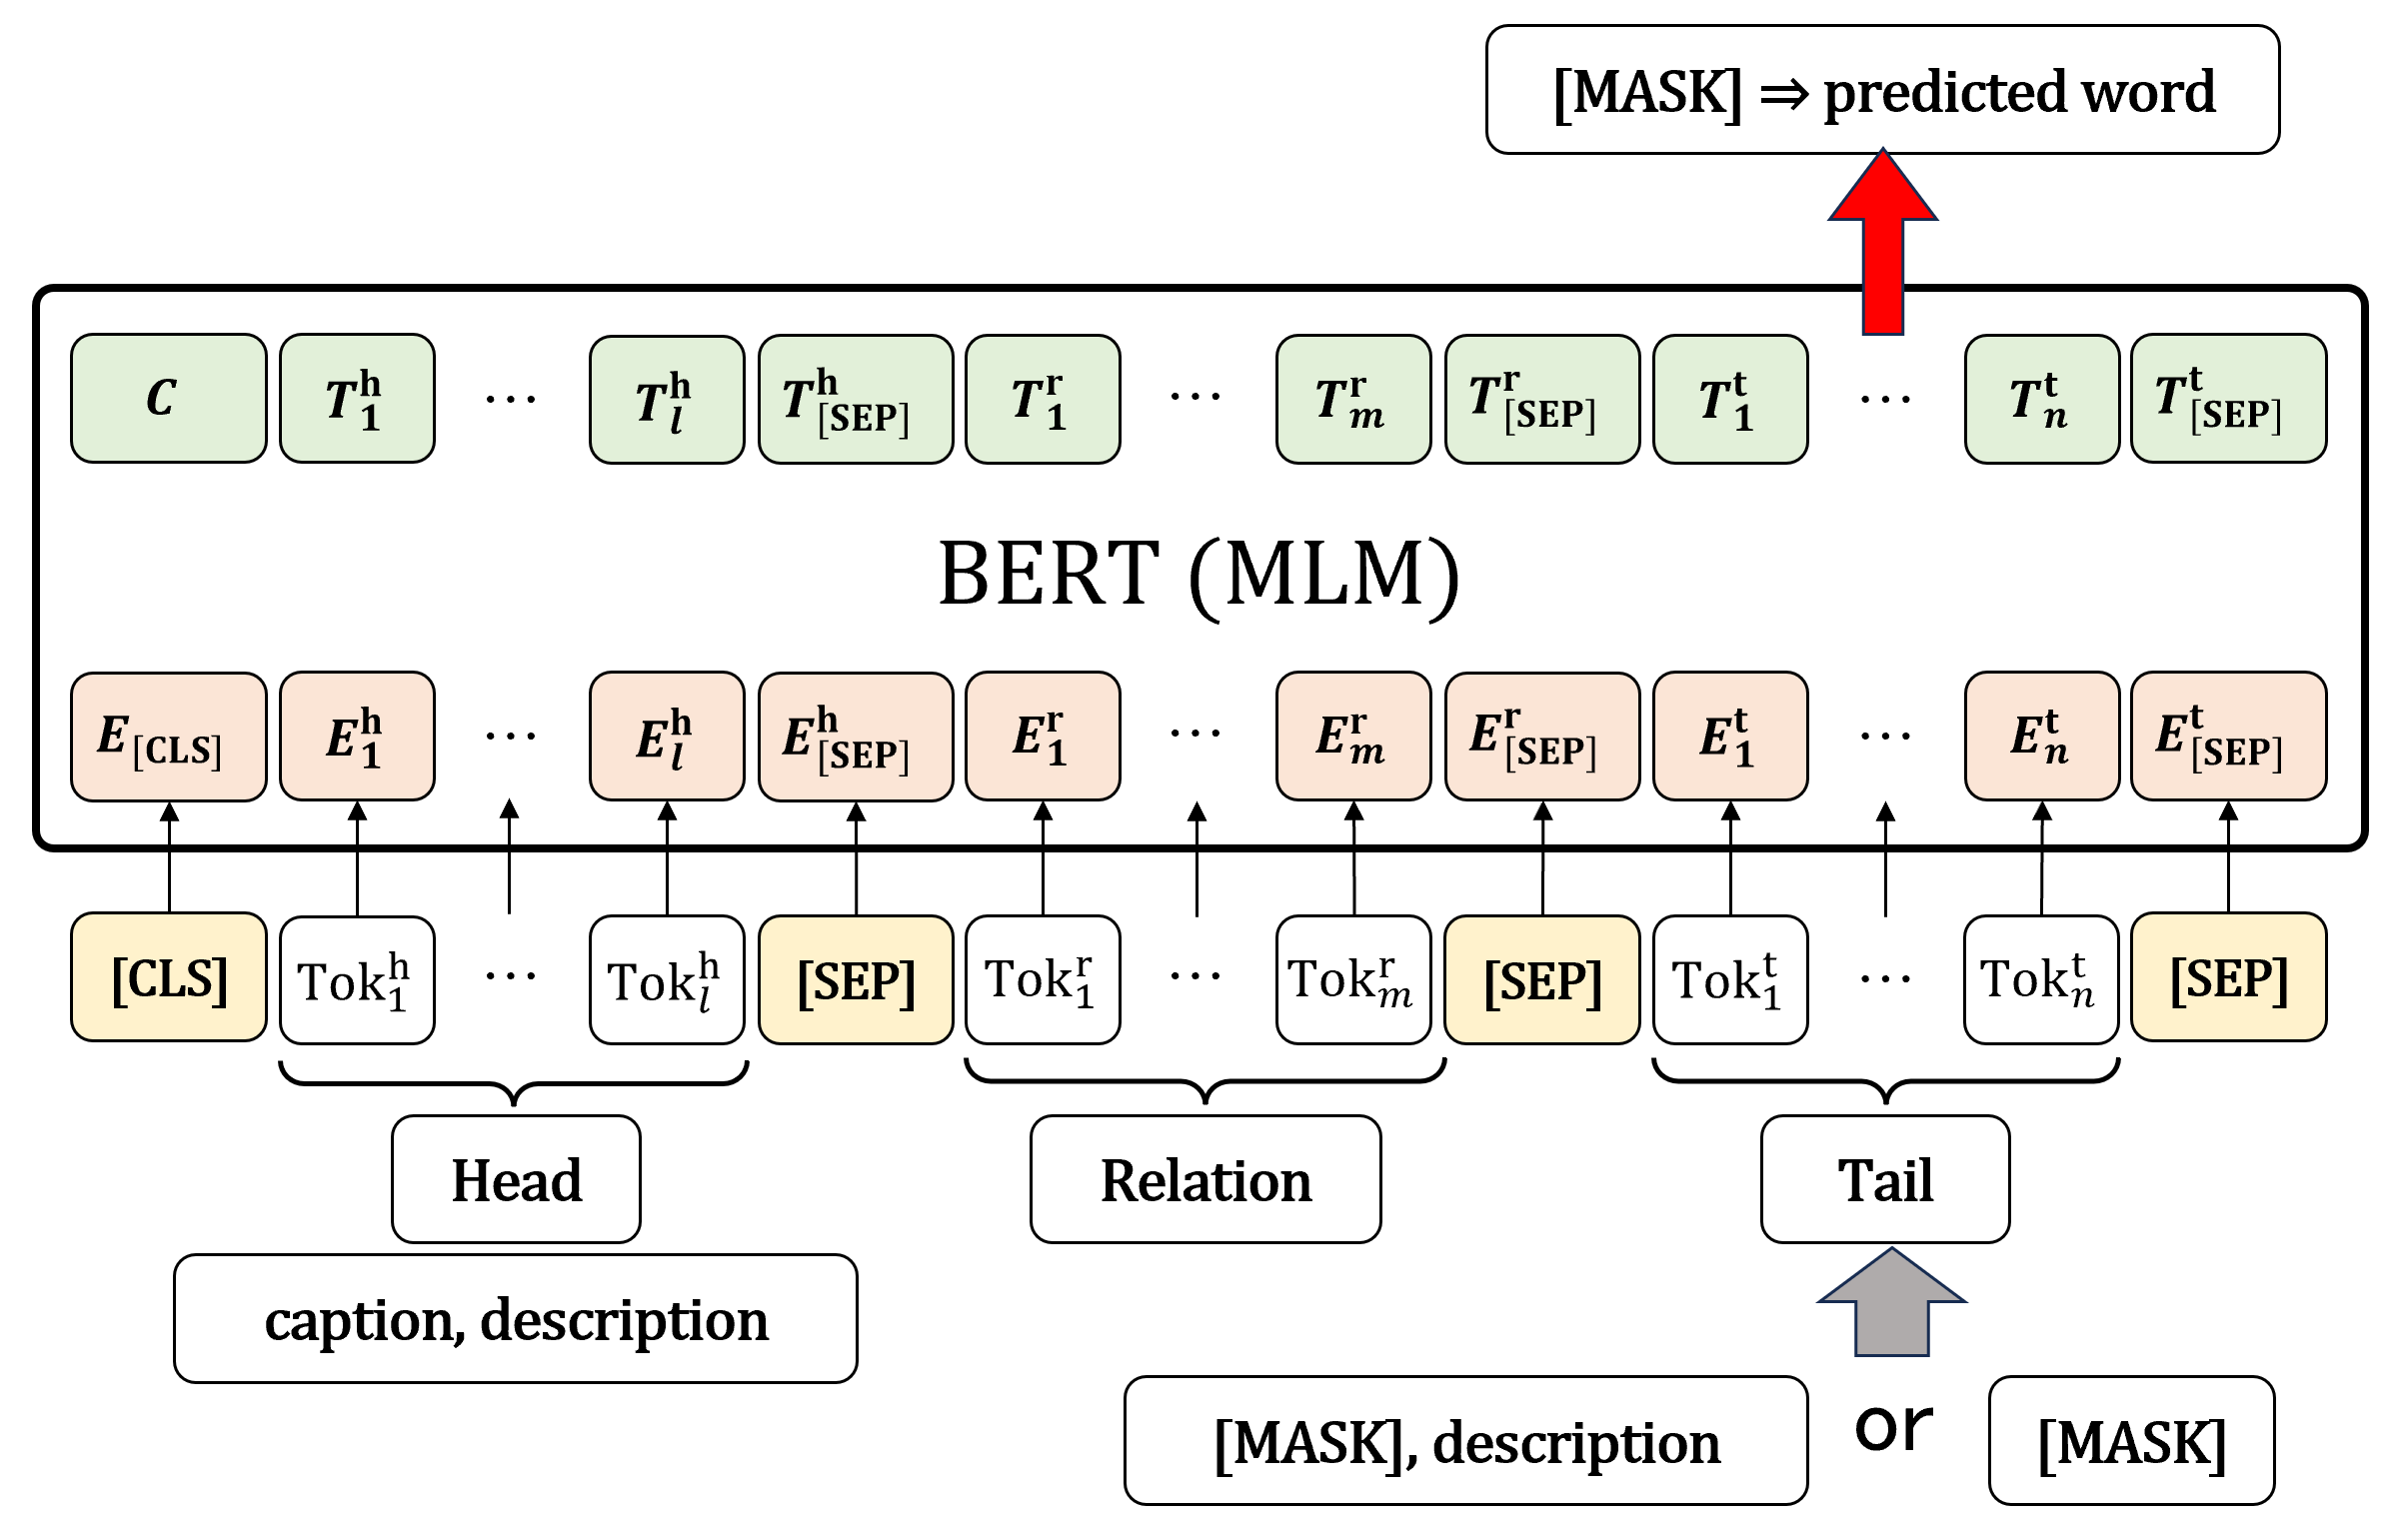
\includegraphics[width=85mm]{assets/KG-MLM.png}
    \vspace{-5mm}
    \caption{提案手法のモデル概略図}
    \label{KG-MLM}
\end{figure}

\begin{figure}[t]
    \centering
    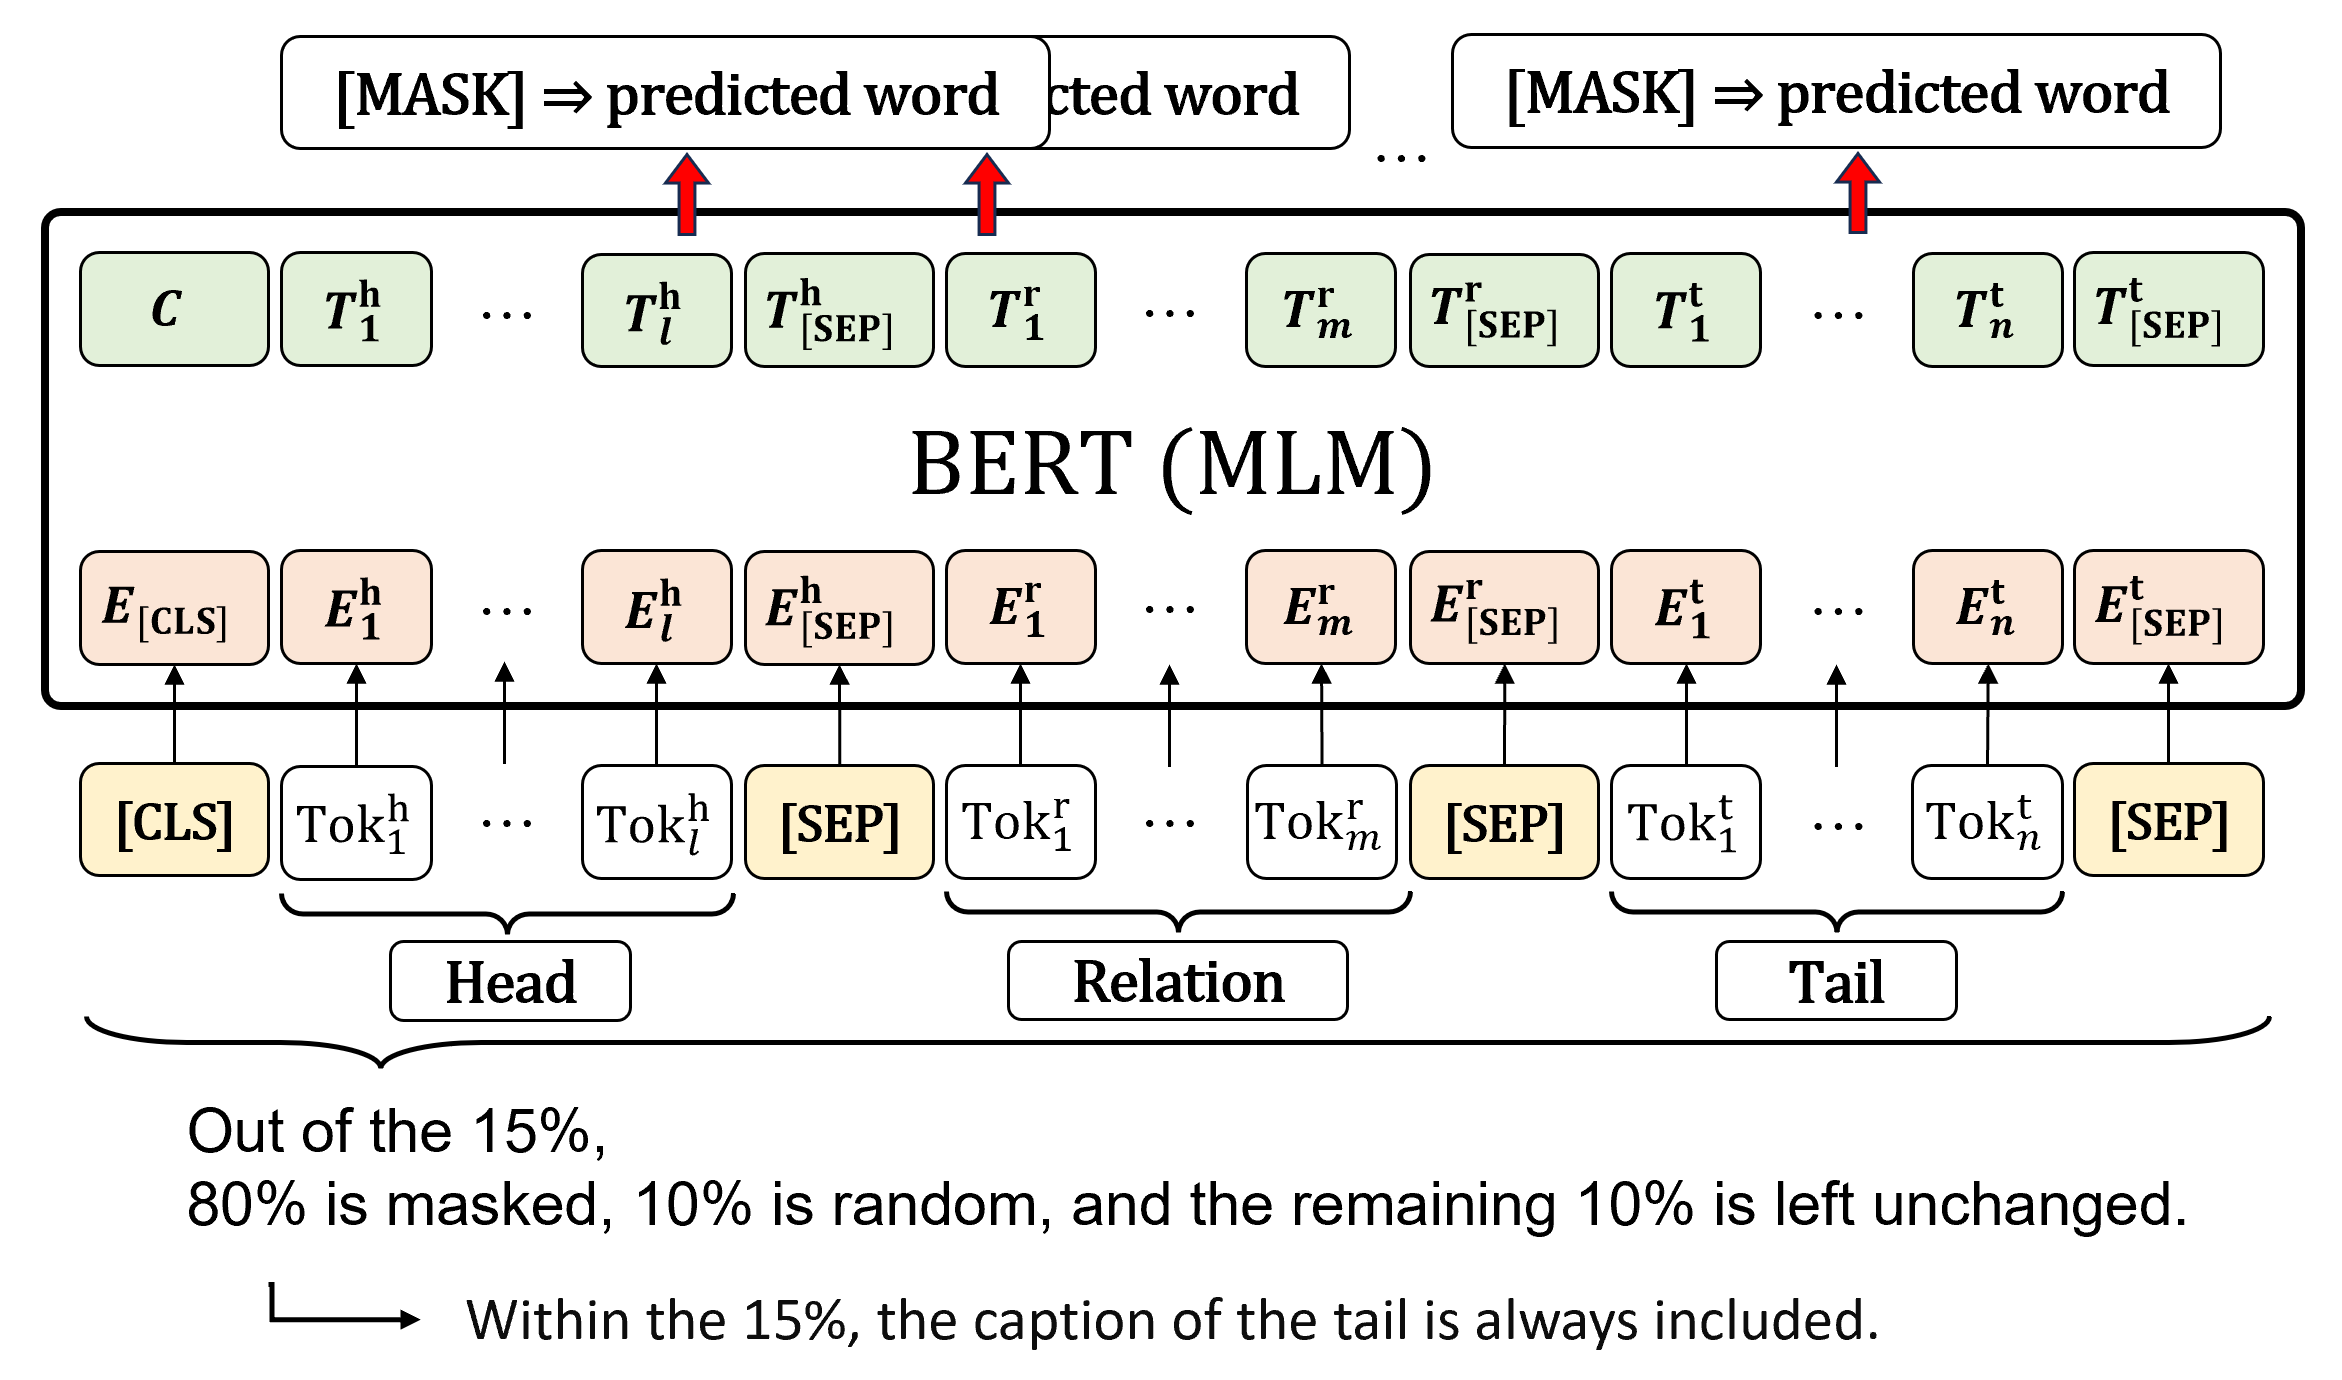
\includegraphics[width=85mm]{assets/MLM_fine-tuning_English.png}
    \vspace{-5mm}
    \caption{BERT の MLM による fine-tuning の概略図}
    \label{MLM_fine_tuning}
\end{figure}

\vspace{-1mm}
\section{実験}

BERT を MLM で fine-tuning したモデルに対して, 2 種類の入力文を用いて実験した. 以下では 2 種類の実験について説明する. 

\vspace{-1mm}
\subsection{実験 1}

実験 1 では, BERT を MLM で fine-tuning したモデルに対して, triple ``[CLS] head [SEP] relation [SEP] tail [SEP]" における tail の見出し語を ``[MASK]" トークンに置き換えた文 ``[CLS] head [SEP] relation [SEP] [MASK], tail の説明文 [SEP]" を 1 つのシーケンスとして入力する. 図 \ref{KG-MLM} において ``Tail" を ``[MASK], description" とした場合である. これにより, ``[MASK]" トークンとなった tail の見出し語を予測する. なお, 予測する tail の見出し語の説明文をそのまま入力しているため, 通常想定される tail 予測タスクより tail の予測が容易である.

\vspace{-1mm}
\subsection{実験 2}

実験 2 では, 実験 1 の入力文 ``[CLS] head [SEP] relation [SEP] [MASK], tail の説明文 [SEP]" における tail の説明文を除去した文 ``[CLS] head [SEP] relation [SEP] [MASK] [SEP]" を 1 つのシーケンスとして入力する. この場合, 図 \ref{KG-MLM} における ``Tail" は ``[MASK]" のみとなる. これにより, ``[MASK]" トークンとなった tail の見出し語を予測する. なお, 予測する tail の見出し語の説明文は入力していないため, head と relation の情報のみを用いて tail を予測する形となる. \par

\vspace{-1mm}
\subsection{評価指標}

評価指標として Mean Reciprocal Rank (MRR), Hits@$k$, Filtered MRR, Filtered Hits@$k$ を用いる. 予測結果の $r$ 番目に正解があるとき, その順位 $r$ のことを rank と呼ぶ. ${\rm |T|}$ を triple 数, ${r}_{i}$ を triple$_{i}$ における正解 tail の rank とすると, MRR は (\ref{MRR}) 式で表される.
\vspace{-1mm}
\begin{equation}
    {\rm MRR} = \frac{1}{\rm |T|} \sum^{\rm |T|}_{i=1} \frac{1}{r_{i}}
    \label{MRR}
\end{equation}
Hits@$k$ は, tail 予測において上位 $k$ 個以内に正解の要素が出力されている割合を表す. このとき, あるテスト triple の正解 tail より予測結果の上位にそのテスト triple と同じ head と relation をもつ triple の tail が存在する場合, その分不当に低くランク付けされる. そこで, テスト triple と同じ head と relation をもつ triple の tail を予測結果から除去してランク付けをする. この rank を Filtered rank とする. 表 \ref{filltered_rank} に例を示す. 表 \ref{filltered_rank} において, テスト triple が (head, relation, word $r$) で, データとして triple (head, relation, word 2), (head, relation, word 4) の 2 つが存在するとき, rank を 2 つ繰り上げることで Filtered rank を得る. Filtered rank によって計算される MRR, Hits@$k$ をそれぞれ Filtered MRR, Filtered Hits@$k$ とする. 本研究では $k=1, 3, 10$ で評価した. MMR, Hits@$k$, Filtered MRR, Filtered Hits@$k$ はすべて値が大きいと推定精度が良いと判断される. \par

\begin{table}[t]
    \centering
    \caption{Filtered rank の例}
    \vspace{-3mm}
    \label{filltered_rank}
    \scalebox{0.90}{
    \begin{tabular}{|c|c|cc|c|} \hline
      triple&rank&\multicolumn{2}{|c|}{tail 予測結果}& Filtered rank \\ \hline \hline
      &1&word 1&&1 \\
      存在&2&word 2&除去& - \\
      &3&word 3&&2 \\
      存在&4&word 4&除去& - \\
      &\vdots & \vdots&& \vdots \\
      正解&$r$ &word $r$ && $r-2$ \\ \hline
    \end{tabular}
    }
\end{table}

\vspace{-1mm}
\subsection{パラメータ}

本研究では WN18RR を訓練データ, 検証データ, テストデータとしてそれぞれ 8 : 1 : 1 に分割して用いた. 表 \ref{num} に WN18RR における entity, relation, triple の数, 訓練データ, 検証データ, テストデータの数を示す. \par
表 \ref{parameta_em} に比較手法の KG-BERT と実験 1, 2 のパラメータを示す. なお, KG-BERT の eval batch size と max seq length は実験環境の都合上文献値とは異なっている. また, 表中の「- (ハイフン)」はそのモデルには必要のないパラメータを表している. \par

\begin{table}[t]
    \centering
    \caption{WN18RR の内訳}
    \vspace{-3mm}
    \label{num}
    \scalebox{1.0}{
    \begin{tabular}{|ccc|ccc|} \hline
        entity & relation & triple & 訓練 & 検証 & テスト \\ \hline \hline
      40,943 & 11 & 93,003 & 86,835 & 3,034 & 3,134 \\ \hline
    \end{tabular}
    }
\end{table}

\begin{table}[t]
    \centering
    \caption{KG-BERT と実験 1, 2 のパラメータ}
    \vspace{-3mm}
    \label{parameta_em}
    \scalebox{1.0}{
    \begin{tabular}{|c|c|c|} \hline
        パラメータ&KG-BERT (文献値)&実験 1, 2 \\ \hline \hline
        leaning rate&$5.0 \times 10^{-5}$&$5.0 \times 10^{-5}$\\
        mask probability&-&0.15\\\
        batch size&32&32\\
        eval batch size&128 (5000)&-\\
        max seq length&32 (50)&128\\
        epoch &5&20\\ \hline
    \end{tabular}
    }
\end{table}

\vspace{-1mm}
\section{実験結果}

\vspace{-1mm}
\subsection{実験 1, 2}

表 \ref{result} に KG-BERT と実験 1, 2 の結果を示す. KG-BERT は本実験と tail 予測方法が異なるため単純な比較はできないが, 参考として文献値と再現実験の 2 つの結果を示している. 表中の「- (ハイフン)」は文献 \cite{KG-BERT} に記載されていなかったことを表している. \par

\begin{table}[t]
    \centering
    \caption{KG-BERT と実験 1, 2 の結果}
    \vspace{-3mm}
    \label{result}
    \scalebox{0.90}{
    \begin{tabular}{|c|cccc|} \hline
        &\multicolumn{4}{|c|}{WN18RR}\\
        モデル&MRR&Hits@1&Hits@3&Hits@10\\ \hline \hline
        KG-BERT (文献値)&-&-&-&52.4\\
        KG-BERT (再現実験)&0.25&12.41&29.44&51.85\\ \hline
        実験 1&0.546&52.55&56.16&57.79\\
        実験 1 (Filtered)&0.550&52.81&56.38&57.82\\ \hline
        実験 2&0.168&10.94&19.37&27.95\\
        実験 2 (Filtered)&0.169&11.04&19.66&28.05\\ \hline
    \end{tabular}
    }
\end{table}

表 \ref{result} より, 実験 1 ではすべての評価指標において KG-BERT の結果を上回る結果が得られた. これにより, tail 予測に BERT の MLM を利用することの有効性が確認できた. しかし, 通常想定される tail 予測タスクより tail の予測が容易であるため, KG-BERT と単純な比較はできない. また, Filtered MRR, Filtered Hits@$k$ について MRR, Hits@$k$ と比較するとその値の変化は微細な範囲にとどまった. \par
実験 2 では Hits@$1$ において KG-BERT と同程度の結果が得られたが, 他の評価指標においては下回る結果となった. また, Filtered MRR, Filtered Hits@$k$ については実験 1 と同様に MRR, Hits@$k$ より少し向上したがほとんど変化しておらず, 訓練データ内の triple の tail 予測もうまくできていないことがわかった. \par

\vspace{-1mm}
\subsection{考察}

実験 1, 2 における tail 予測結果について考察する. \par
% 以下では triple を (``head の見出し語, その説明文", ``relation", ``tail の見出し語, その説明文") とし, tail の見出し語を太字で表す. 
実験 1 でテスト triple (``position, the particular portion of space occupied -", ``hypernym", ``point, the precise location of something; a spatially limited location; ``she walked to a point where she could survey the whole street"") の見出し語 ``point" を ``[MASK]" に置き換えて tail を予測すると, 提案手法では ``point" を予測して正解したのに対し, KG-BERT では ``situation" を予測していた. これは tail の見出し語の説明文に ``point" が含まれていることが予測に影響を与えたと考えられる. そのため, tail の説明文の情報が結果に大きく影響することがわかった. \par
実験 2 でテスト triple (``evidence, an indication that makes something evident; -", ``hypernym", ``indication, something that serves to indicate or suggest; -") の見出し語 ``indication" とその説明文を ``[MASK]" に置き換えて tail を予測すると, 提案手法では ``indication" を予測して正解したのに対し, KG-BERT では ``averment" を予測していた. これは head の見出し語の説明文に ``indication" が含まれていることが予測に影響を与えたと考えられる. このような head の見出し語の説明文に tail の情報を含む triple に対して提案手法は有効であることがわかった.\par

\vspace{-1mm}
\section{まとめと今後の課題}
本研究では, MLM を用いた 2 種類の入力文に対する tail 予測について KG-BERT と比較し, 実験 1 において KG-BERT を上回る結果が得られた. また, 実験 2 では提案手法が head の見出し語の説明文に tail の情報を含む triple に対して有効であることがわかった. BERT の MLM を用いた Knowledge Graph 補完において, 学習していない見出し語でも head と relation と説明文のような前後の文章から適切に予測することができたため, Knowledge Graph 補完手法としての有効性が確認できた. \par
今後の課題として, MLM の出力候補を entity に限定したモデルの作成, head 予測や relation 予測への応用が挙げられる. \par

\section*{謝辞}
本研究は,日本学術振興会科学研究補助金基盤研究 (C) (課題番号 23K11252) の補助を得て行われたものである.

\bibliographystyle{jsai}
\bibliography{index}

\end{document}
